\documentclass{article}
\usepackage{booktabs}            % For better looking tables
\usepackage[a4paper, margin=1in]{geometry}  % Adjusts margins
\usepackage{titling}             % For cover page formatting
\usepackage{caption}             % Allows caption alignment
\usepackage{graphicx}            % For including images
\usepackage{listings}            % For source code listings
\usepackage{xcolor}              % For color definitions
\usepackage{enumitem}            % For customizing list formatting
\usepackage[hidelinks]{hyperref} % For clickable links and TOC
\usepackage{float}               % To force figure placement using [H]
\usepackage{fancyhdr}            % For custom headers/footers
\usepackage{amsmath, amssymb}    % For math symbols
\usepackage[acronym]{glossaries}

% \makeglossaries


% Fancyhdr setup for a professional header/footer
\pagestyle{fancy}
\fancyhf{}
\lhead{\textbf{PPH7021F - Assignment 2}}

\rhead{Jolene Wium}
\cfoot{\thepage}

% Listings settings for Python code
\lstset{
    language=Python,
    basicstyle=\ttfamily\small,
    numbers=left,
    numberstyle=\tiny,
    stepnumber=1,
    numbersep=10pt,
    backgroundcolor=\color{white},
    frame=single,
    breaklines=true,
    postbreak=\mbox{\textcolor{red}{$\hookrightarrow$}\space},
}

% Listings settings for Python code
% \lstset{
%     language=Python,
%     basicstyle=\ttfamily\small,
%     numbers=left,
%     numberstyle=\tiny,
%     stepnumber=1,
%     numbersep=10pt,
%     backgroundcolor=\color{white},
%     frame=single,
%     breaklines=true,
%     postbreak=\mbox{\textcolor{red}{$\hookrightarrow$}\space},
% }

% Allow numbering down to paragraphs (simulate subsubsubsections)
\setcounter{secnumdepth}{4}

\begin{document}

\begin{titlepage}
    \begin{center}
        \vspace*{3cm}
            
        \Huge
        \textbf{PPH7021F Assignment 2}
            
        \vspace{1.5cm}

        \huge
            
        \textbf{Jolene Wium}                      % <-- author
        \vspace{1cm}
        \Large


        WMXJOL001
            
        % \vfill
        
        \texttt{WMXJOL001\_dataset.csv}
            
        \vspace{1cm}
            
        % \includegraphics[width=0.4\textwidth]{logo-hkust.png}
        % \\
        
        \Large
        
        \today
            
    \end{center}
\end{titlepage}
\newpage
\newpage
% === PLAGIARISM DECLARATION ===

\begin{center}
    {\LARGE \textbf{Declaration of Plagiarism}}
\end{center}

\vspace{2cm}

\noindent I, \textbf{Jolene Wium}, hereby declare that this assignment is my own work. It has not been submitted for any other course or degree, and all sources I have used or quoted have been indicated and acknowledged by means of complete references.

\vspace{2cm}

\noindent\textbf{Signature:} \rule{10cm}{0.4pt}

\vspace{1cm}

\noindent\textbf{Date:} \rule{10cm}{0.4pt}

\newpage
\newpage
% Table of Contents
\tableofcontents
\newpage

% List of Tables, Figures, and Listings
\listoftables
% \newpage
\listoffigures
% \newpage
% \lstlistoflistings
\newpage
\section[q1]{Question 1}
\subsection{Question 1.a}
\textit{In a single table reporting relevant descriptive statistics in the overall sample
and by year [as a categorical variable, pick two years to perform the analysis].
Include summary statistics as you did in assignment 1. However, you should
include p-values in your table assessing the difference in the following variables
by year.}
\begin{table}[ht]
    \centering
    \begin{tabular}{lcccc}
        \toprule
        Variable & Overall & 2015 & 2020 & P-value \\
        \midrule
        pm10\_concentration & 34.20 ± 36.41 & 37.76 ± 39.33 & 30.78 ± 33.03 & 0.00000 \\
        pm25\_concentration & 13.91 ± 15.25 & 15.11 ± 18.13 & 12.98 ± 12.53 & 0.00925 \\
        no2\_concentration & 15.90 ± 10.61 & 18.16 ± 11.52 & 14.20 ± 9.52 & 0.00000 \\
        pm25\_tempcov & 87.73 ± 22.05 & 86.04 ± 22.99 & 89.17 ± 21.12 & 0.00783 \\
        \bottomrule
\end{tabular}
\caption{Descriptive statistics for WHO regions overall and by year}
\end{table}




\subsection{Question 1.b}
\textit{Write a short paragraph describing any differences you observe in the above
variables across the two years you have selected to analyse}

\begin{itemize}
    \item The mean pm10 concentration decreased from 37.76 in 2015 to 30.78 in 2020. The P-Value shows that we  reject the null hypothesis, indicating that the difference is statistically significant with a p-value of 0.00000.
    \item The mean pm25 concentration also decreased from 15.11 in 2015 to 12.98 in 2020, with a p-value of 0.00925.
    \item The mean no2 concentration showed a notable decrease from 18.16 in 2015 to 14.20 in 2020, with a p-value of 0.00000.
    \item The pm25 temporal coverage increased slightly from 86.04 in 2015 to 89.17 in 2020, with a p-value of 0.00783.
\end{itemize}

\newpage
\section[Question 2]{Question 2}
\textit{Examine whether there is an association between year (as a categorical variable, pick
two years to perform the analysis) and pm25\_concentration.}

\subsection{Question 2.a}
\textit{Is this an analysis of paired or independent samples? Explain your answer.}\\

\noindent Independent samples. The locations included in each year differ. There are 288 more cities in 2020 than in 2015. If the question related to picking one city and comparing the $PM_{2.5}$ in 2015 and 2020, then it would be a paired sample.



\subsection{Question 2.b}
\textit{Check assumptions and apply an appropriate statistical test to test whether
there is a difference in pm25\_concentration across the two years you have
selected.}

\paragraph*{Step 1: Check for Normality}
To determine if the data is parametric or non-parametric, the Shapiro-Wilk test was used to check for normality.

\begin{itemize}
    \item $H_0$: The population is normally distributed.
    \item $H_A$: The population is not normally distributed.
\end{itemize}

The results of the Shapiro-Wilk test indicate that both $p$-values are very small ($p < 0.05$). Therefore, we reject $H_0$ and conclude that the data is not normally distributed.

\paragraph*{Step 2: Apply the Mann-Whitney U Test}
Since the data is not normally distributed, the Mann-Whitney U test was used to compare the two years.

\begin{itemize}
    \item $H_0$: $\mu_1 = \mu_2$ (The medians of the two years are equal.)
    \item $H_A$: $\mu_1 \neq \mu_2$ (The medians of the two years are not equal.)
\end{itemize}

The Mann-Whitney U test yielded a $p$-value of $< 0.05$. Therefore, we reject $H_0$ and conclude that there is a significant difference in $PM_{2.5}$ concentration between the two years.


\newpage
\section[q3]{Question 3}
\textit{Is there an association between year [as a continuous variable, use all years to perform
the analysis] and pm25\_concentration.}

\subsection{Question 3.a}
\textit{Plot a single graph/figure showing the relationship between these two variables.}

\begin{figure}[H]
    \centering
    % 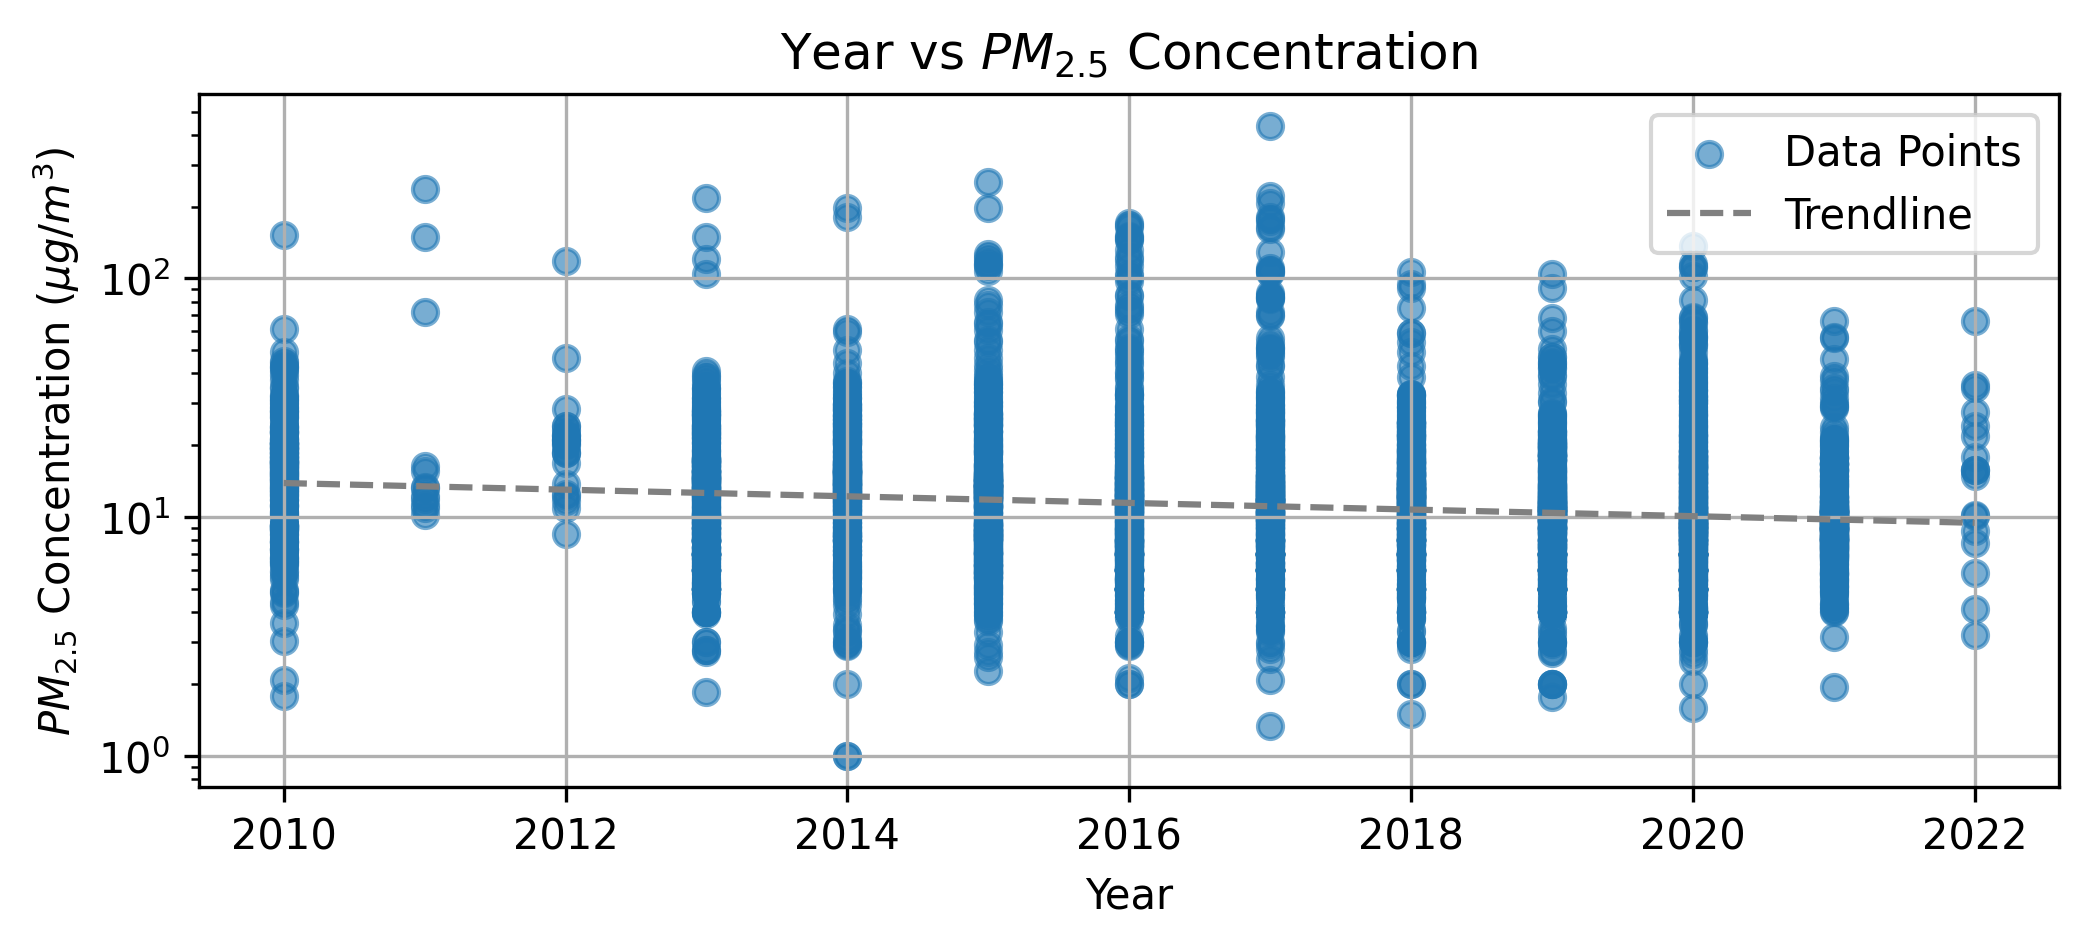
\includegraphics[width=\textwidth]{img/q3_year_vs_pm25log.png}
    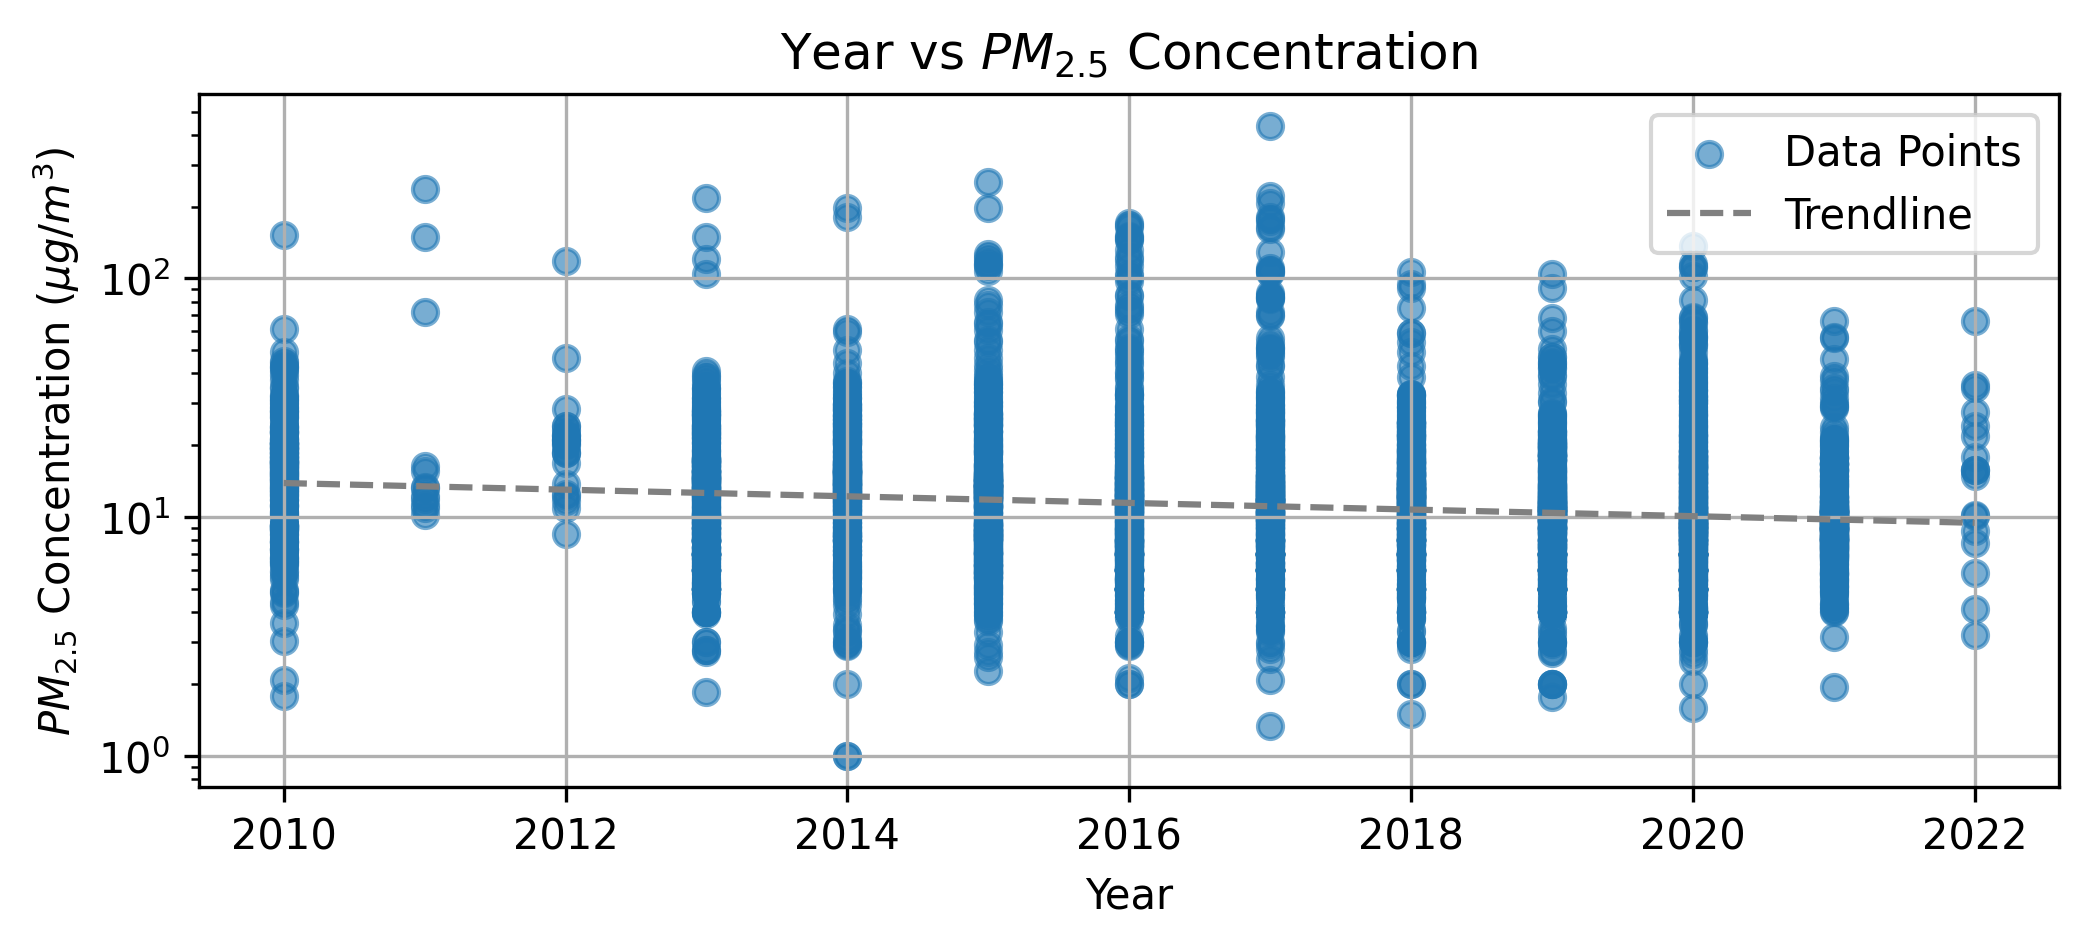
\includegraphics[width=0.8\textwidth]{img/q3_year_vs_pm25log.png}
    \caption{Relationship between year and $PM_{2.5}$ concentration.}
    \label{fig:year_pm25_relationship}
\end{figure}


\subsection{Question 3.b}
\textit{Select an appropriate statistical test for correlation.
Check the assumptions of your chosen statistical test for correlation. Report
your decisions on the validity of the assumptions for your chosen statistical test. Justify your decisions.
Report the name of the final test you choose to run}

\paragraph*{Step 1: Check for normality}
Year is ordinal data. Although it is used as contnuous data for the correlation test, it will not be normall distributed.  Normality of To determine of $PM_{2.5}$ concentration has already been tested in question 2 using the Shapiro-Wilk test.

\begin{itemize}
    \item $H_0$: $PM_{2.5}$ concentration is normally distributed.
    \item $H_A$: $PM_{2.5}$ concentration is not normally distributed.
\end{itemize}

The $p$-value of the Shapiro-Wilk test is $< 0.05$. Thus, we reject $H_0$ and conclude that the data is not normally distributed.

\paragraph*{Step 2: Check for monotonicity}
The scatterplot in Figure \ref{fig:year_pm25_relationship} shows a negative correlation between year and $PM_{2.5}$ concentration. The data points appear to follow a general downward trend and suggests that the relationship is monotonic.

Since neither variable is normally distributed and the data is monotonic, the Spearman rank correlation coefficient is used to determine a correlation coefficient.


\subsection{Question 3.c}
\textit{Run your chosen test, report the p-value and report on the magnitude and
direction of the effect (use the test results and refer to your figure from 3a).}

The Spearman rank correlation coefficient is used to determine the correlation between year and $PM_{2.5}$ concentration. The code used to determine the Spearman rank correlation are shown in Listing \ref{lst:pm25year}.
The Spearman rank correlation coefficient is $-0.163$, indicating a weak negative correlation between year and $PM_{2.5}$ concentration. The $p$-value is $< 0.05$, indicating a that there is a monotonic relationship between year and $PM_{2.5}$ concentration that is not by chance. This slight negative slant can be seen by the grey line in Figure \ref{fig:year_pm25_relationship}.\\

\begin{lstlisting}[caption={Python code to evaluate correlation between $PM_{2.5}$ concentration and year}, label={lst:pm25year}]
    spearman_corr, spearman_pval = spearmanr(years, pm25)

    print(f"Spearman's correlation: {spearman_corr}")
    print(f"P-value: {spearman_pval}")
\end{lstlisting}

\newpage
\section[Question 4]{Question 4}
\textit{Air pollution exhibits significant geospatial variation across the globe. Investigate if
there is an association in your sample between pm10\_concentration and who\_region
[pick a single year in which to investigate the association]. }

\subsection{Question 4.a}
\textit{Plot an appropriate figure/graph to visualise the relationship between these
two variables. } \\

\noindent Figure \ref{fig:q4_box_pm10_region} shows a box and whiskers plot to show the spread of points between the six WHO regions for 2020.

\begin{figure}[H]
    \centering
    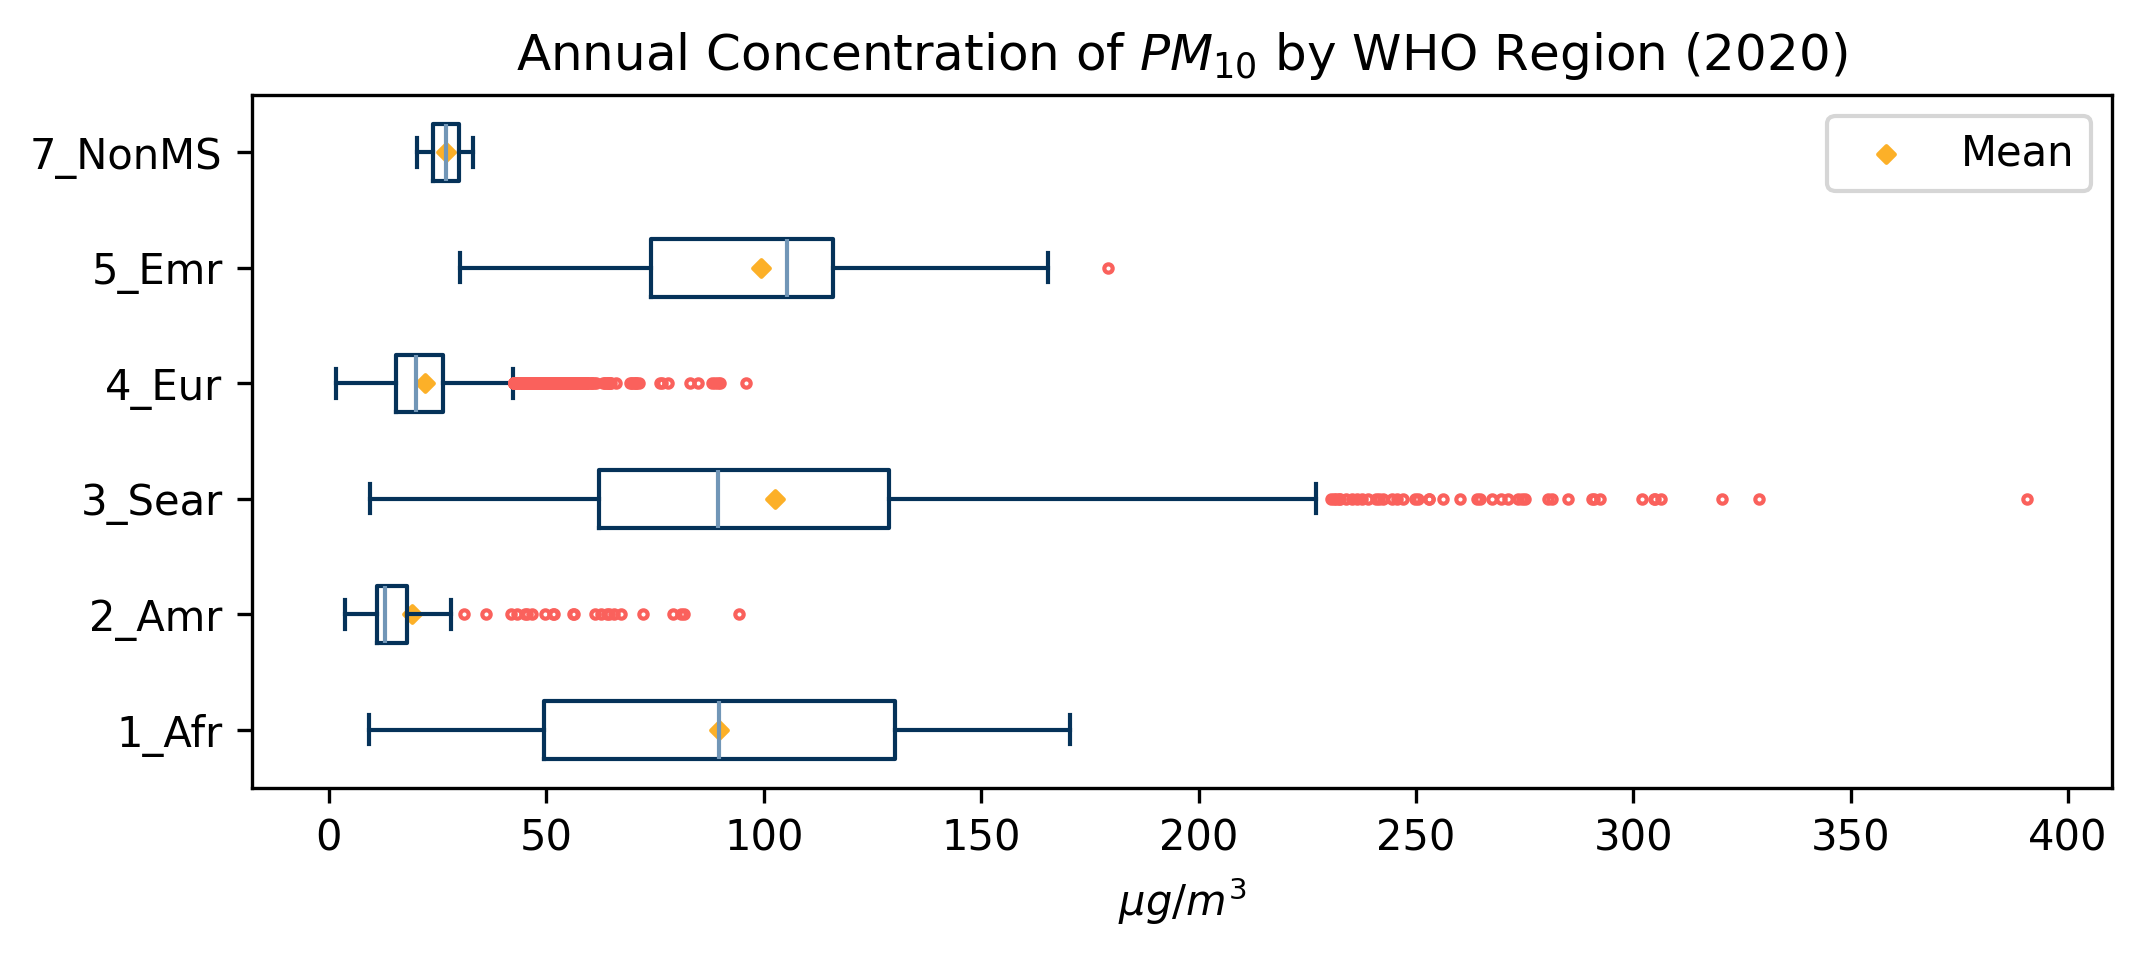
\includegraphics[width=0.8\textwidth]{img/q4_box_pm10_region.png}
    \caption{$PM_{10}$ concentration by WHO region - 2020.}
    \label{fig:q4_box_pm10_region}
\end{figure}

\subsection{Question 4.b}
\textit{Select an appropriate statistical test to test if there is a difference in pm10\_concentration
by who\_region (if in doubt consult the flow charts on Amathuba).
How many groups are being compared and are they paired or independent
groups? Check the assumptions of your chosen statistical test. Report your decisions
on the validity of the assumptions for your chosen statistical test. Justify your
decisions. Report the name of the final test you choose to run.}\\

\noindent Six independent groups are being compared (`1\_Afr', `2\_Amr', `3\_Sear', `4\_Eur', `5\_Emr', `7\_NonMS'). The groups are independent because the $PM_{10}$ concentrations in each region are not related to each other. 

\noindent The data are not normally distributed, as indicated by the Shapiro-Wilk test results. Therefore, the Kruskal-Wallis test (non-parametric alternative of ANOVA) was chosen to compare the median $PM_{10}$ concentrations across the different WHO regions. 


\subsection{Question 4.c}
\textit{Run your chosen test, report the p-value and use your sample data to report
on the direction and magnitude of the effect (use the test results and refer to
your figure from 3a) }

\noindent The Kruskal-Wallis test was used to determine if there is a difference in $PM_{10}$ concentration across the six WHO regions. 


\begin{itemize}
    \item $H_0$: Mean $PM_{10}$ concentration is the same accross all six WHO regions.
    \item $H_A$: Mean $PM_{10}$ concentration is not the same accross all six WHO regions.
\end{itemize}
% The code used to determine the Kruskal-Wallis test is shown in Listing \ref{lst:pm10region}. 

\noindent The Kruskal-Wallis test yielded a $p$-value of 0.00 ($p < 0.05$). Thus, we reject $H_0$ and conclude that there is a difference in $PM_{10}$ concentration means between the six WHO regions. The mean $PM_{10}$ concentration by region is represented by the yellow dots in Figure \ref{fig:q4_box_pm10_region}. 

% \begin{lstlisting}[caption={Python code to evaluate $PM_{10}$ concentration accross six WHO regions}, label={lst:pm10region}]
%     from scipy.stats import kruskal
   
%     statistic, p_value = kruskal(*data_by_region)

% \end{lstlisting}


\newpage
\section[q5]{Question 5}
\textit{Assessing whether air pollution levels are above the WHO recommended guidelines
is imperative for determining the association between health and air pollution at a
population level. Is there an association between who\_region and the air pollution
exposure categories created in Assignment 1 [pick a single year in which to investig-
ate the association]?}

\subsection{Question 5.a}
\textit{Plot a single bar graph showing the relationship between these two variables.}\\

In 2020, only four regions submitted $PM_{2.5}$ concentration data to the WHO.  Figure \ref{fig:q5_bar_pm25_region} shows the $PM_{2.5}$ concentration categories by WHO region for 2020. The regions are colour-coded according to the air pollution exposure categories created in Assignment 1.

\begin{figure}[H]
    \centering
    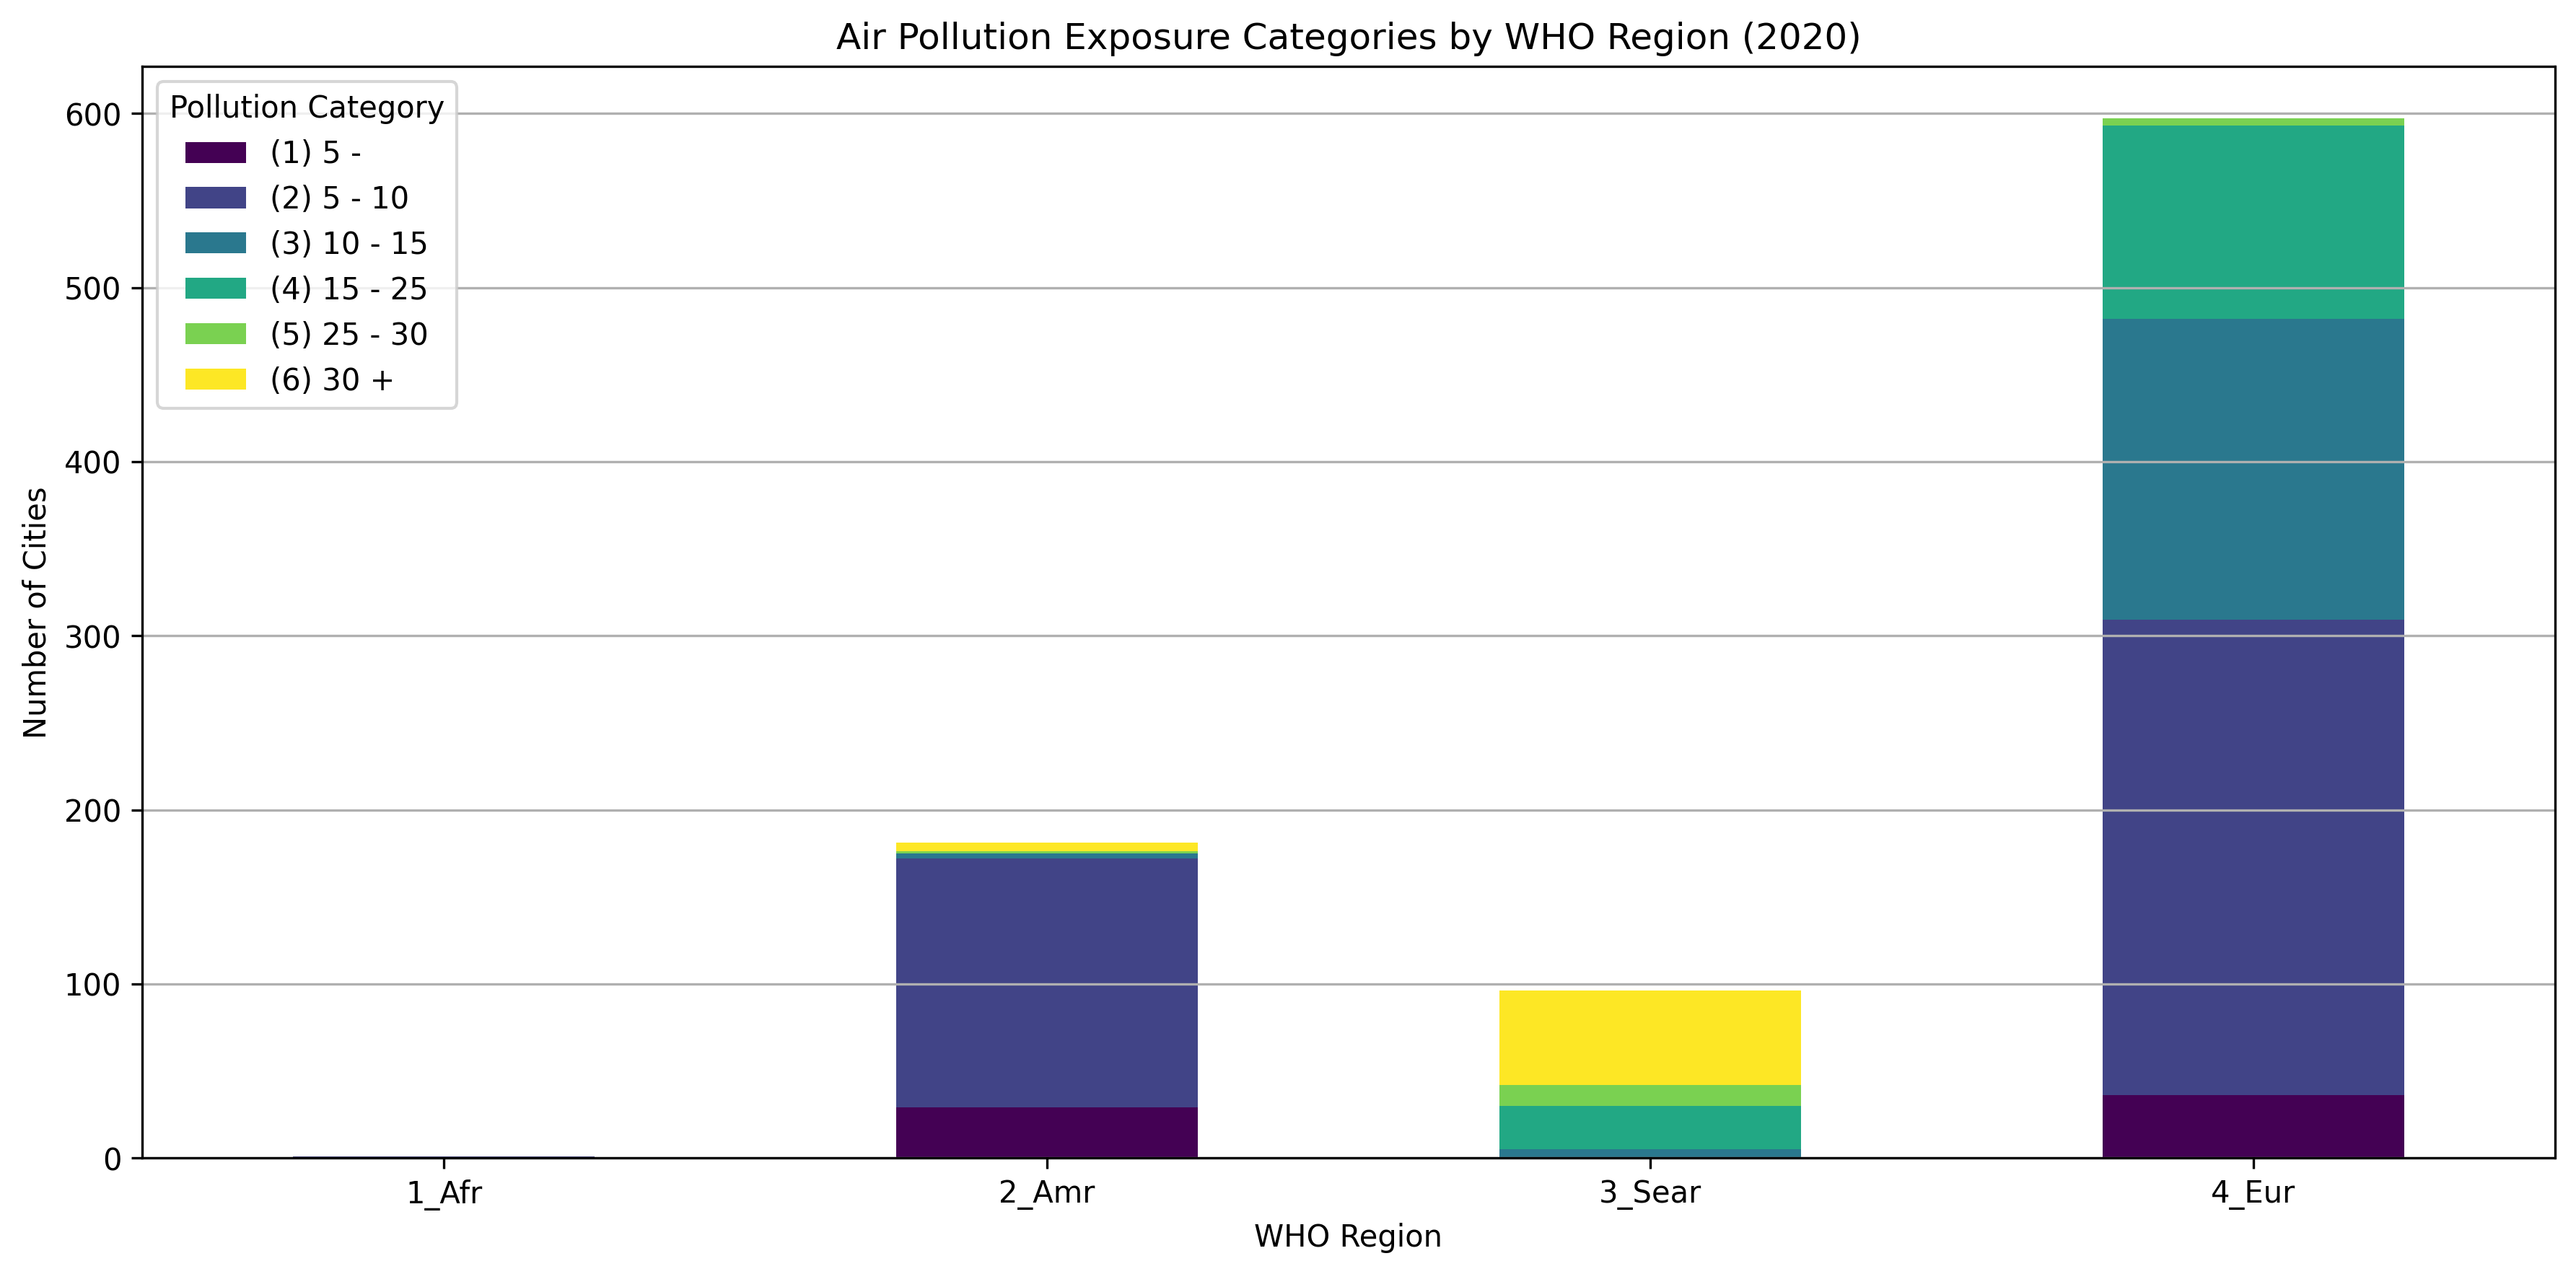
\includegraphics[width=0.8\textwidth]{img/q5_bar_pm25_region.png}
    \caption{$PM_{2.5}$ concentration by WHO region - 2020.}
    \label{fig:q5_bar_pm25_region}
\end{figure}

\subsection{Question 5.b}
\textit{What is the prevalence of the highest air pollution exposure category you created?}
\begin{itemize}
    \item \textit{In your overall sample?}
    \item \textit{In the 4\_Eur who\_region?}
    \item \textit{In the 1\_Afr who\_region?}
\end{itemize}

\textit{Report your answers in written sentences (not just reporting number). Hint: refer to your descriptive table or make a new 2x2 table to help you answer this.}


% \begin{tabular}{lrrrrrrr}
%     \toprule
%     pm25\_cats & (1) 5 - & (2) 5 - 10 & (3) 10 - 15 & (4) 15 - 25 & (5) 25 - 30 & (6) 30 + & Total \\
%     who\_region &  &  &  &  &  &  &  \\
%     \midrule
%     1\_Afr & 0 & 1 & 0 & 0 & 0 & 0 & 1 \\
%     2\_Amr & 29 & 143 & 3 & 0 & 1 & 5 & 181 \\
%     3\_Sear & 0 & 0 & 5 & 25 & 12 & 54 & 96 \\
%     4\_Eur & 36 & 273 & 173 & 111 & 4 & 0 & 597 \\
%     Total & 130 & 834 & 362 & 272 & 34 & 118 & 1750 \\
%     \bottomrule
%     \caption{Descriptive statistics for WHO regions overall and by year}
% \end{tabular}\\

\begin{table}[ht]
    \centering
    \begin{tabular}{lrrrrrrr}
        \toprule
        pm25\_cats & (1) 5 - & (2) 5 - 10 & (3) 10 - 15 & (4) 15 - 25 & (5) 25 - 30 & (6) 30 + & Total \\
        who\_region &  &  &  &  &  &  &  \\
        \midrule
        1\_Afr & 0 & 1 & 0 & 0 & 0 & 0 & 1 \\
        2\_Amr & 29 & 143 & 3 & 0 & 1 & 5 & 181 \\
        3\_Sear & 0 & 0 & 5 & 25 & 12 & 54 & 96 \\
        4\_Eur & 36 & 273 & 173 & 111 & 4 & 0 & 597 \\
        Total & 130 & 834 & 362 & 272 & 34 & 118 & 1750 \\
        \bottomrule
\end{tabular}
\caption{Descriptive statistics for WHO regions overall and by year}
\end{table}



\begin{enumerate}
    \item \textit{In the overall sample} The prevalence of the highest air pollution exposure category (30+) in the overall sample is 118/1750 = 6.74\%.
    \item \textit{In the 4\_Eur who\_region?} The prevalence of the highest air pollution exposure category (30+) in the 4\_Eur region is 0/597 = 0\%.
    \item \textit{In the 1\_Afr who\_region?} The prevalence of the highest air pollution exposure category (30+) in the 1\_Afr region is 0/1 = 0\%.
\end{enumerate}

\subsection{Question 5.c}
\textit{Calculate the prevalence ratio for the relationship between the highest air pol-
lution exposure category you created and who\_region, specifically the 4\_Eur
and 1\_Afr regions. Interpret the prevalence ratio. 
• Be sure to specify which region (4\_Eur or 1\_Afr) you are treating as the
exposed and unexposed groups. Your outcome should be the highest air
pollution exposure category you created.
• You can calculate the confidence interval in the software or by hand using
the formula provided in the measures of association slides}




\newpage
\section[q6]{Question 6}
\textit{We are concerned that population size might modify the relationship between who\_region
and the highest air pollution exposure category you created. Determine if there is
any evidence of effect modification.}

\subsection{Question 6.a}
\textit{Create either a single table or multiple tables to summarise the relationship
between who\_region and highest air pollution exposure category you cre-
ated, grouped by population size category you created in Assignment 1.
If you have more than 3 population size categories, use the first three categories
for this analysis.}

\subsection{Question 6.b.i}
\textit{Investigate whether the relationship between who\_region and highest air pol-
lution exposure category you created varies by population size category you
created in Assignment 1. Be sure to specify which groups (4\_Eur or 1\_Afr)
you are treating as the exposed and unexposed groups. Your outcome should
be highest air pollution exposure category you created.}

\subsubsection{Question 6.b.ii}
\textit{To do this, calculate the prevalence ratio in the three population size cat-
egories (you can do this by hand or in your software).
Report whether the association between who\_region and highest air
pollution exposure category you created is statistically significant in each
of the three population size categories by using 95\% confidence intervals
or by conducting chi-squared tests of the association in each of the three
groups. Write out your answer for each group in a sentence (do not just
report the numbers).}


\subsubsection{Question 6.b}
\textit{Does population size appear to be modifying the effect of who\_region
on highest air pollution exposure category you created? Justify your an-
swer using the information and results calculated above. (3)
Biostatistics 1: Assignment 2 5 of 6}

\subsection{Question 6.c}
\textit{Based on your analysis and interpretation above, select which of the results
from the list below you would report in your manuscript and why.}

\subsubsection{Question 6.c.i}
\textit{Just the crude overall prevalence ratio.}

\subsubsection{Question 6.c.ii}
\textit{The stratified prevalence ratios (in each population category).}

\subsubsection{Question 6.c.iii}
\textit{An adjusted prevalence ratio like the Mantel Haenszel adjusted association (adjusted for population category).
Hint: You need to filter your data to include just one population category at a time then do the next population category to do these grouped
analyses
}


\newpage

\end{document}
